\lecture{11}{Entropy and Heat}{Qiang Zhu}{scribe-name1,2,3}


\section{Chemical Potential}
When we talk a system of Ideal gas), it is decribed by the following fundamental parameters, $T,P,N$,
\begin{enumerate}
\item uneven $T$ $\rightarrow$ heat     flow ($S \uparrow$), we call it {\it thermal equilibrium}
\item uneven $P$ $\rightarrow$ pressure flow ($S \uparrow$), we call it {\it mechanical equilibrium}
\item uneven $N$ $\rightarrow$ particle flow ($S \uparrow$), we call it ~~~~~~~~~~~~~?
\end{enumerate}
\begin{figure}[h]
\centering
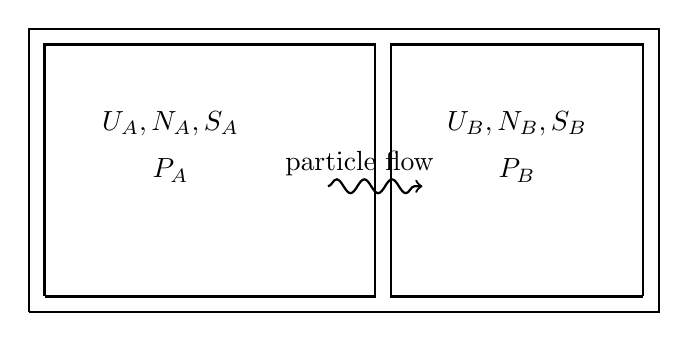
\begin{tikzpicture}[thick]
\draw (0,0.4) -- (8,0.4) -- (8,4) -- (0,4) -- (0,0.4);
\draw (0.2,0.6) -- (4.4,0.6) -- (4.4,3.8) -- (0.2,3.8) -- (0.2,0.6);
\node at (1.8,2.8) {$U_A, N_A, S_A$};
\node at (1.8,2.2) {$P_A$};
\draw (7.8,0.6) -- (4.6,0.6) -- (4.6,3.8) -- (7.8,3.8) -- (7.8,0.6);
\node at (6.2,2.8) {$U_B, N_B, S_B$};
\node at (6.2,2.2) {$P_B$};
\draw [->,decorate,decoration=snake] (3.8,2) -- (5.0,2) node [above, xshift=-0.8cm]{particle flow};
\end{tikzpicture}
\caption{A schematic particle flow between two gases.}
\end{figure}

Such process due to the exchange of particles is called {\it diffusion}. Since diffusion is also a
spontaneous process. It must lead to the increase of entropy (recall we have learned the mixing entropy).
This indicates that $S$ is also a function of $N$ (as we learned in Chapter 2).
Therefore, we can also derive the equilibrium condition for diffusion (analogy to $P$).
\begin{equation} \label{entropy} 
\frac {\partial{S_A}} {\partial{N_A}} =  \frac {\partial{S_B}} {\partial{N_B}} 
\end{equation}

What's the physical meaning of $\partial{S_A}/\partial{N_A}$? \\
If we dig a bit on the units, we will find $\partial{S_A}/\partial{V_A}$ has a unit of J/K. 
Not a very pleasant quantity. Let's multiply it by $-T$ so that it has the dimension of energy.
\begin{equation} \label{entropy} 
\mu = -T (\frac {\partial{S}} {\partial{N}})_{U,V}
\end{equation}

So it means the equilibrium condition for diffusive process is $\mu_A$ = $\mu_B$.

Now let's we generalize the processes which I shown in the beginning.
\begin{enumerate}
\item uneven $T(\frac {\partial{S}} {\partial{U}} = 1/T)  $ $\rightarrow$ heat     flow ($S\uparrow$) , we call it {\it thermal equilibrium.}
\item uneven $P(\frac {\partial{S}} {\partial{V}} = P/T)  $ $\rightarrow$ pressure flow ($S\uparrow$) , we call it {\it mechanical equilibrium.}
\item uneven $N(\frac {\partial{S}} {\partial{N}} = \mu/T)$ $\rightarrow$ particle flow ($S\uparrow$) , we call it {\it diffusive equilibrium.}
\end{enumerate}

\section{The Generalized Thermodynamic Identity}

\begin{equation} dS = (\frac{\partial S}{\partial U})dU 
                    + (\frac{\partial S}{\partial V})dV  
                    + (\frac{\partial S}{\partial N})dN 
\end{equation}
\begin{equation} dS = \frac{1}{T}dU
                    + \frac{P}{T}dV  
                    - \frac{\mu}{T}dN
\end{equation}
\begin{equation} dU = TdS - PdV  + \mu dN\end{equation}
\begin{enumerate}
\item $\Delta{U}$ = 0 , $\Delta{V}$=0, $\mu$=
\item $\Delta{U}$ = 0 , $\Delta{V}$=0, $\mu$=
\end{enumerate}
$\mu$ is the system's energy change when you add one particle while $S$ and $V$ is fixed. Normally, $\mu$ is negative.\\
\begin{equation} dU = TdS - PdV  + \sum_{\substack{i}} \mu_i dN_i\end{equation}


\section{Chemical potential for Einstein Solid}

\begin{figure}[h]
\centering
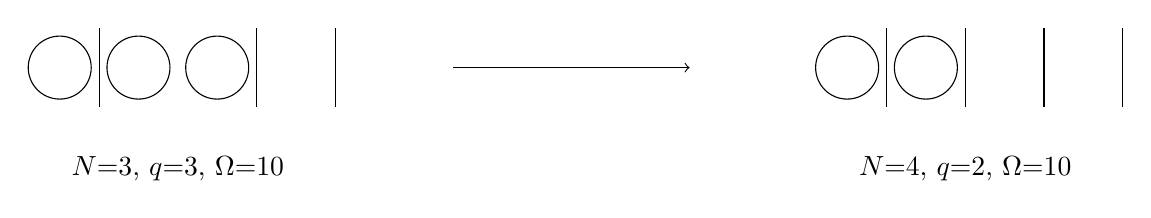
\begin{tikzpicture}
\draw (2,0) circle (0.4cm);
\draw (2.5,-0.5) -- (2.5,0.5);
\draw (3,0) circle (0.4cm);
\draw (4,0) circle (0.4cm);
\draw (4.5,-0.5) -- (4.5,0.5);
\draw (5.5,-0.5) -- (5.5,0.5);
\draw (3.5,-1.0) node [below] {$N$=3, $q$=3, $\Omega$=10};
\draw [->] (7.0,0.0) -- (10.0,0.0);
\draw (12,0) circle (0.4cm);
\draw (12.5,-0.5) -- (12.5,0.5);
\draw (13,0) circle (0.4cm);
\draw (13.5,-0.5) -- (13.5,0.5);
\draw (14.5,-0.5) -- (14.5,0.5);
\draw (15.5,-0.5) -- (15.5,0.5);
\draw (13.5,-1.0) node [below] {$N$=4, $q$=2, $\Omega$=10};
\end{tikzpicture}
\end{figure}

For Einstein solid, $\mu$=-$\epsilon$\\\\\\\
\begin{equation} \mu = (\frac{\partial U}{\partial N})_{S,V}  \end{equation}


\section{Chemical potential for ideal gas}

For a more realistic example, let's do ideal gas 
\begin{equation} \label{entropy} 
S = Nk[\text{ln}(\frac{V}{N} (\frac{4\pi m U}{3Nh^2})^{3/2}) + \frac{5}{2}]
\end{equation}

Differentiating with respect to $N$ gives
\begin{equation}
\begin{split}
\mu =& -T{ k[\text{ln} (V (\frac{4\pi mU}{3h^2})^{3/2} )  - \text{ln}N^{5/2} + \frac{5}{2} ] - NK\frac{5}{2}\frac{1}{N} }\\
    =& -kT\text{ln}[\frac{V}{N} (\frac{4{\pi} mU}  {3Nh^2})^{3/2} ]\\
    =& -kT\text{ln}[\frac{V}{N} (\frac{2{\pi} mkT} {h^2})^{3/2} ]
\end{split}
\end{equation}
Note that here $U = 3/2NKT$ was used in the last step.

He (0.32 eV, how to calculate?)
Ar (0.42 eV, how to calculate?)


\begin{enumerate}
\item Mixing 1 mol He with 1 mol He (both at standard condition)
\item Mixing 1 mol He with 1 mol Ar (both at standard condition)
%\item No diffusion Einstein Solid.
%\item No diffusion between two He gases.
%\item generalized equation
\end{enumerate}


\section{Exercise}
Problem 3.37. Consider a monoatomic ideal gas that lives at a height $z$ above sea level, so each molecule has potential energy $mgz$ 
in addition to it kinetic energy.\\
(a) Show that the chemical potential is the same as if the gas were at sea level plus $mgz$
\begin{equation}
  \mu  = -kT\text{ln}[\frac{V}{N} (\frac{2{\pi} mkT} {h^2})^{3/2} ] + mgz
\end{equation}
\\\\\\\\\\\\





(b) Suppose you have two chunks of He gas, one at sea level, and one at height $z$, each having the same temperature and volume.
Assuming that they are in diffusive equilibrium, show that the number of molecules in the higher chunk is
\begin{equation}
  N(z)  = N(0)e^{-mgz/kT}
\end{equation}
\\\\\\\\\\


\section{Homework}
Problem 3.36, 3.37, 3.38

